%%%%%%%%%%%%%%%%%%%%%%%%%%%%%%%%%%%%%%%%%
% Jacobs Landscape Poster
% LaTeX Template
% Version 1.1 (14/06/14)
%
% Created by:
% Computational Physics and Biophysics Group, Jacobs University
% https://teamwork.jacobs-university.de:8443/confluence/display/CoPandBiG/LaTeX+Poster
%
% Further modified by:
% Nathaniel Johnston (nathaniel@njohnston.ca)
%
% This template has been downloaded from:
% http://www.LaTeXTemplates.com
%
% License:
% CC BY-NC-SA 3.0 (http://creativecommons.org/licenses/by-nc-sa/3.0/)
%
%%%%%%%%%%%%%%%%%%%%%%%%%%%%%%%%%%%%%%%%%

%----------------------------------------------------------------------------------------
%	PACKAGES AND OTHER DOCUMENT CONFIGURATIONS
%----------------------------------------------------------------------------------------

\documentclass[final]{beamer}

\usepackage[scale=1.24]{beamerposter} % Use the beamerposter package for laying out the poster

\usetheme{confposter} % Use the confposter theme supplied with this template

\setbeamercolor{block title}{fg=ngreen,bg=white} % Colors of the block titles
\setbeamercolor{block body}{fg=black,bg=white} % Colors of the body of blocks
\setbeamercolor{block alerted title}{fg=white,bg=dblue!70} % Colors of the highlighted block titles
\setbeamercolor{block alerted body}{fg=black,bg=dblue!10} % Colors of the body of highlighted blocks
% Many more colors are available for use in beamerthemeconfposter.sty

%-----------------------------------------------------------
% Define the column widths and overall poster size
% To set effective sepwid, onecolwid and twocolwid values, first choose how many columns you want and how much separation you want between columns
% In this template, the separation width chosen is 0.024 of the paper width and a 4-column layout
% onecolwid should therefore be (1-(# of columns+1)*sepwid)/# of columns e.g. (1-(4+1)*0.024)/4 = 0.22
% Set twocolwid to be (2*onecolwid)+sepwid = 0.464
% Set threecolwid to be (3*onecolwid)+2*sepwid = 0.708

\newlength{\sepwid}
\newlength{\onecolwid}
\newlength{\twocolwid}
\newlength{\threecolwid}
\setlength{\paperwidth}{48in} % A0 width: 46.8in
\setlength{\paperheight}{36in} % A0 height: 33.1in
\setlength{\sepwid}{0.024\paperwidth} % Separation width (white space) between columns
\setlength{\onecolwid}{0.22\paperwidth} % Width of one column
\setlength{\twocolwid}{0.464\paperwidth} % Width of two columns
\setlength{\threecolwid}{0.708\paperwidth} % Width of three columns
\setlength{\topmargin}{-0.5in} % Reduce the top margin size
%-----------------------------------------------------------

\usepackage{graphicx}  % Required for including images

\usepackage{booktabs} % Top and bottom rules for tables

%\setbeamercolor{block alerted title}{fg=white,bg=norange} % Change the alert block title colors
%\setbeamercolor{block alerted body}{fg=black,bg=white} % Change the alert block body colors

%----------------------------------------------------------------------------------------
%	TITLE SECTION
%----------------------------------------------------------------------------------------

\title{A best-practices model for cyberinfrastructure collaboration \\ \large used to create the Coupled RipCAS-DFLOW model for floodplain modeling} % Poster title

\author{Matthew A. Turner$^{a,b}$, Sarah Miller$^{c,d}$, Angela Gregory$^e$,
        Smriti Chaulagain$^e$, Lucas J. Sheneman$^a$,
        Mark Stone$^e$, Daniel Cadol$^c$
} % Author(s)

\institute{$^a$Northwest Knowledge Network, University of Idaho, USA;
           $^b$Cognitive and Information Sciences, University of California, Merced, USA \\
           $^c$Department of Earth and Environmental Sciences, New Mexico Tech, USA;
           $^d$Environmental Laboratory, U.S. Army Engineer Research and Development Center, Vicksburg \\
           $^e$Department of Civil Engineering, University of New Mexico, USA
           } % Institution(s)

%----------------------------------------------------------------------------------------

\begin{document}

\addtobeamertemplate{block end}{}{\vspace*{2ex}} % White space under blocks
\addtobeamertemplate{block alerted end}{}{\vspace*{2ex}} % White space under highlighted (alert) blocks

\setlength{\belowcaptionskip}{2ex} % White space under figures
\setlength\belowdisplayshortskip{2ex} % White space under equations

\begin{frame}[t] % The whole poster is enclosed in one beamer frame

\begin{columns}[t] % The whole poster consists of three major columns, the second of which is split into two columns twice - the [t] option aligns each column's content to the top

\begin{column}{\sepwid}\end{column} % Empty spacer column

\begin{column}{\onecolwid} % The first column

%----------------------------------------------------------------------------------------
%	OBJECTIVES
%----------------------------------------------------------------------------------------

\begin{alertblock}{Project Goal}
Build a sustainable, easy-to-use, transparent modeling system for riparian zone flood modeling over
many years of successive flood events.
\end{alertblock}
\begin{alertblock}{Poster Objectives}

\begin{itemize}
    \item Introduce basic principles of effective software development, customized for small-team scientific/cyberinfrastructure collaboration
    \item Demonstrate how these principles resulted in an open-source coupled-model system that includes
        automatic data management: Coupled RipCAS-DFLOW (CoRD)
\end{itemize}

\end{alertblock}

%----------------------------------------------------------------------------------------
%	INTRODUCTION
%----------------------------------------------------------------------------------------

\begin{block}{Minimal Solution}
    \begin{itemize}
        \item Write adapters so data from each model is compatible with the other
        \item Create a way to run the coupled modeling system
        \item Write documentation on how to use the adapters
    \end{itemize}
\end{block}

\begin{block}{Deeper Problem}
    \begin{itemize}
        \item Scientists specialize in analysis including scripting, not cyberinfrastructure
        \item Too often developers don't know or appreciate scientists goals and skills
        \item Without open modeling software, it's difficult for models to be externally verified
        \item Modeling results often emerge from highly opaque parameter tunings, limiting the opportunities
            for other scientists to verify results
        \item Too often cyberinfrastructure collaborations lack iterative feedback and progress
        %\item Tools built without scientist participation frequently languish
    \end{itemize}

\end{block}




%------------------------------------------------

%----------------------------------------------------------------------------------------

\end{column} % End of the first column

\begin{column}{\sepwid}\end{column} % Empty spacer column

\begin{column}{\twocolwid} % Begin a column which is two columns wide (column 2)

    \begin{alertblock}{Coupled RipCAS-DFLOW (CoRD) In Action}
        \begin{figure}
            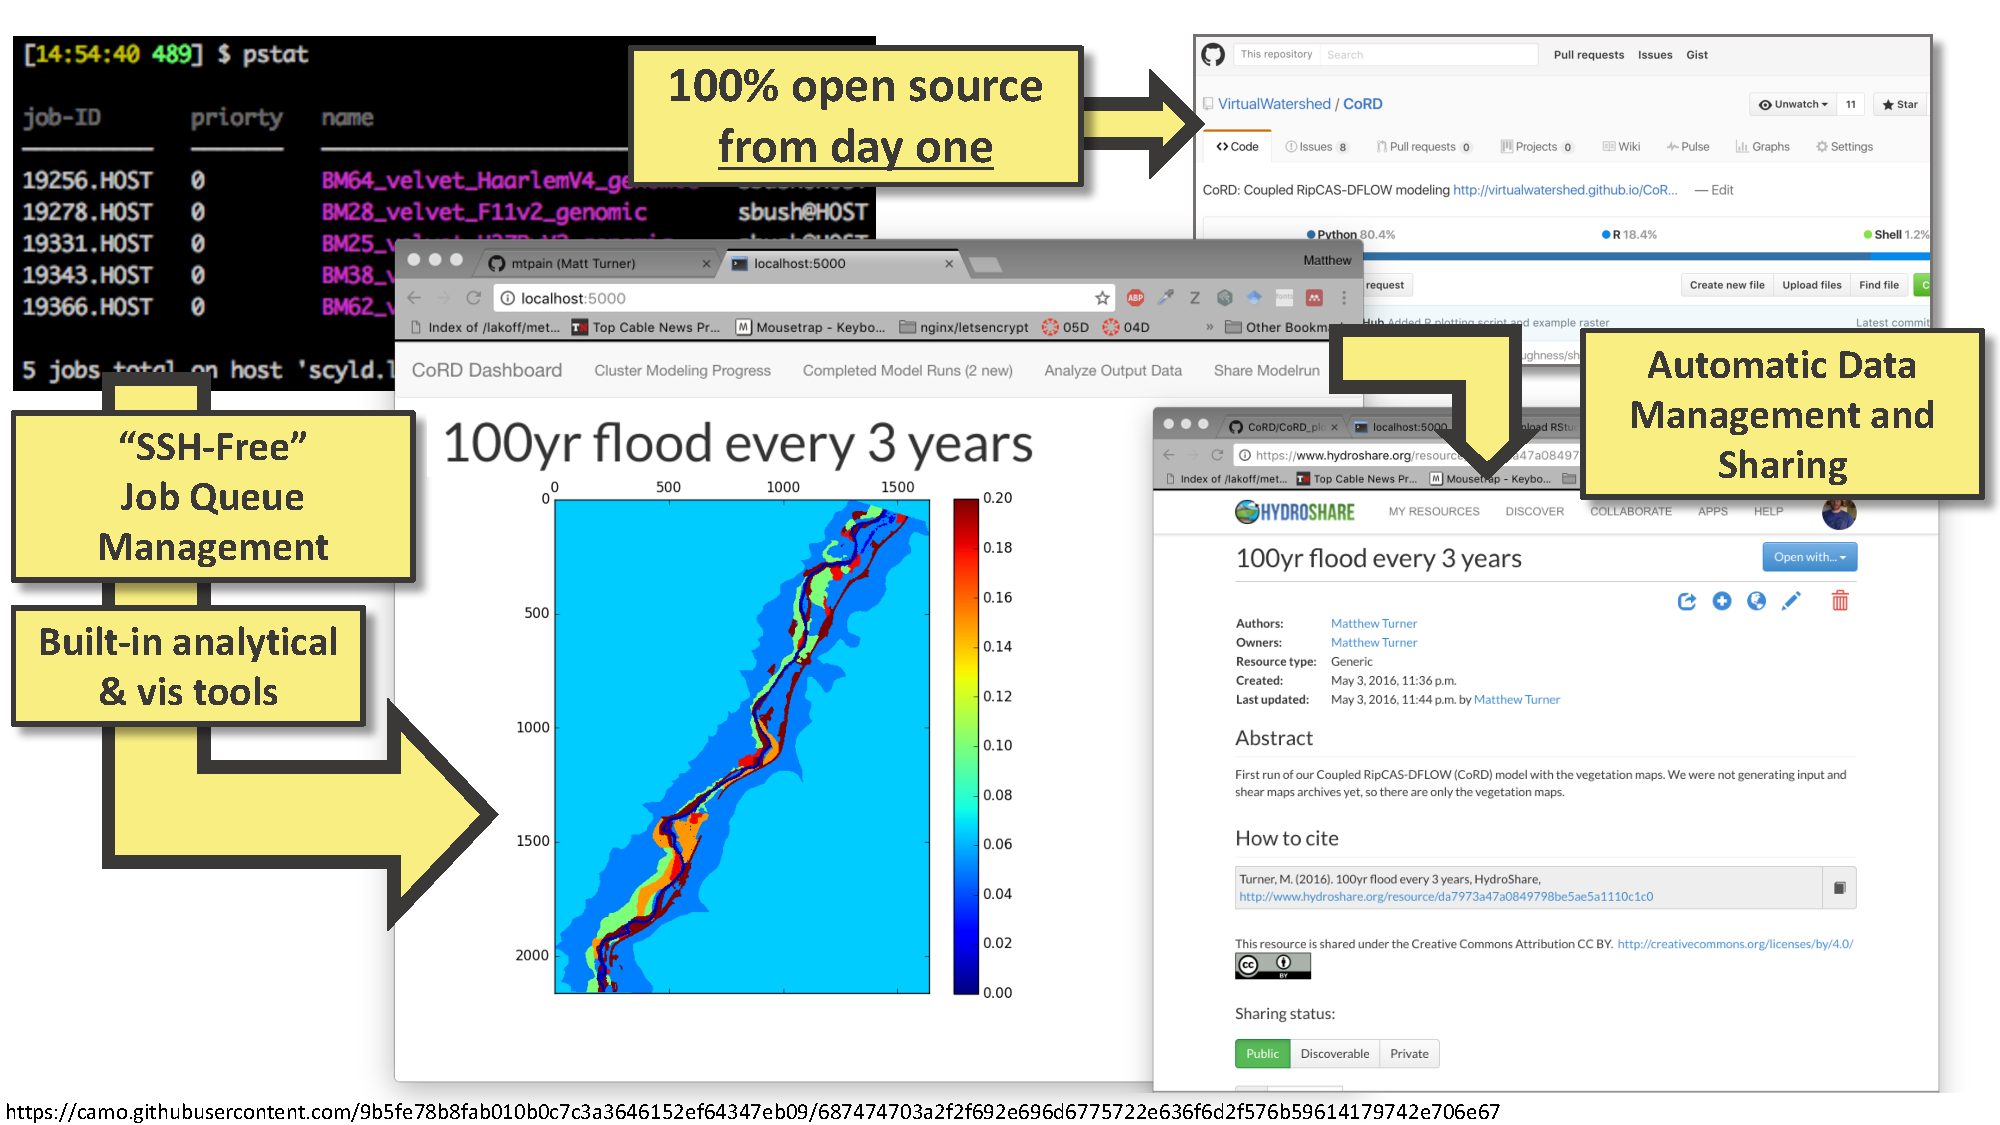
\includegraphics[width=0.8\linewidth]{Figure1.pdf}
            \caption{CoRD couples two models: DFLOW for flood modeling and
            newly developed RipCAS, the Riparian Community Alteration and
            Succession model. HydroShare\cite{Horsburgh2016} provides data
            management via their REST API \cite{HydroShare2016}}
        \end{figure}
    \end{alertblock}

    \vspace{1in}

    \begin{alertblock}{Collaboration}
         
        \begin{figure}
            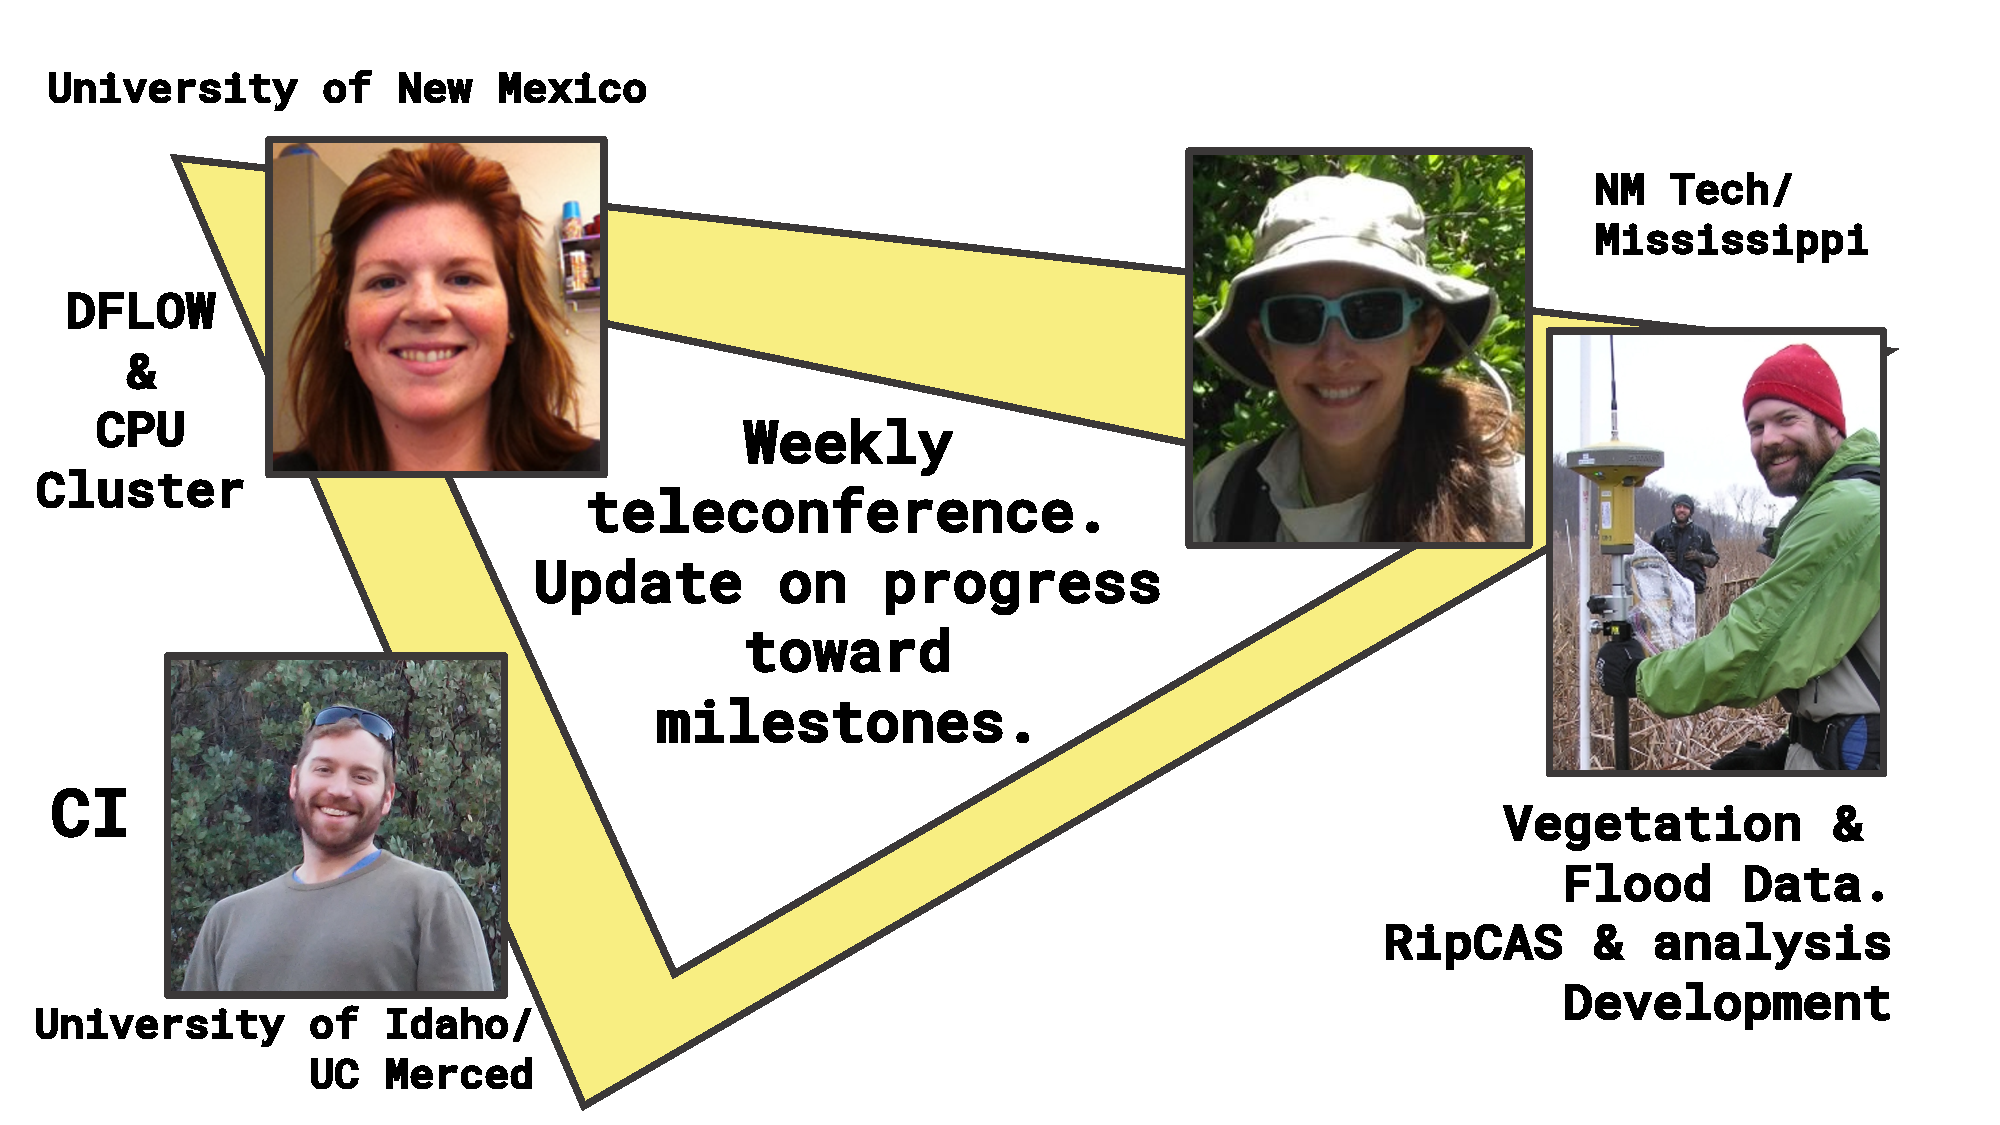
\includegraphics[width=0.6\linewidth]{Figure2.pdf}
            \caption{Our week-to-week team consists of one 
        software developer and 
        four hydrologists. By working towards
        milestones, our work remained focused and progress could be
        clearly measured. GitHub even provides milestones for projects,
        so open software and good practices are easily integrated.}
        \end{figure}
    \end{alertblock}

\end{column} % End of the second column

\begin{column}{\sepwid}\end{column} % Empty spacer column

\begin{column}{\onecolwid} % The third column

%----------------------------------------------------------------------------------------
%	CONCLUSION
%----------------------------------------------------------------------------------------

\begin{block}{Some Key Best Practices}
    \begin{enumerate}
        \item{Work closely with scientists as development partners; commit to weekly meetings}
        \item{Deliver scientifically valuable software quickly in small chunks}
        \item{Do not increase the amount of programming or technical skill required for scientists to do their jobs.}
        \item{Openness is key: open-source software, built-in data management and data sharing.}
        \item{Take an adaptive approach; avoid waterfall planning.}
    \end{enumerate}
\end{block}

\begin{block}{Discussion}
    Monolithic projects like EarthCube and CSDMS are laudable efforts. But 
    EarthCube ``is facing a mid-life crisis,''
    according to a recent report in Science. After five years, an external 
    advisory panel ``warned that EarthCube
    still lacked a clear definition and might not be sustainable\cite{Witze2016}.''
    CSDMS requires a large investment without a guaranteed payoff.
    Modern software development theory predicts that such ``waterfall'' 
    approaches to software are susceptible to slowness \cite{Sutherland2014}.
\end{block}

%----------------------------------------------------------------------------------------
%	ADDITIONAL INFORMATION
%----------------------------------------------------------------------------------------

%\begin{block}{Additional Information}
%
%Maecenas ultricies feugiat velit non mattis. Fusce tempus arcu id ligula varius dictum.
%\begin{itemize}
%\item Curabitur pellentesque dignissim
%\item Eu facilisis est tempus quis
%\item Duis porta consequat lorem
%\end{itemize}
%
%\end{block}

%----------------------------------------------------------------------------------------
%	REFERENCES
%----------------------------------------------------------------------------------------

\begin{block}{References}

\small{\bibliographystyle{unsrt}
\bibliography{bib}\vspace{0.75in}}

\end{block}

%----------------------------------------------------------------------------------------
%	CONTACT INFORMATION
%----------------------------------------------------------------------------------------

%
%\begin{alertblock}{Contact Information}
%
%\begin{itemize}
%\item Web: \href{http://www.university.edu/smithlab}{http://www.university.edu/smithlab}
%\item Email: \href{mailto:john@smith.com}{john@smith.com}
%\item Phone: +1 (000) 111 1111
%\end{itemize}
%
%\end{alertblock}
%
%\begin{center}
%\begin{tabular}{ccc}
%\includegraphics[width=0.4\linewidth]{logo.png} & \hfill & \includegraphics[width=0.4\linewidth]{logo.png}
%\end{tabular}
%\end{center}
%
%%----------------------------------------------------------------------------------------
%
\end{column} % End of the third column
%
\end{columns} % End of all the columns in the poster

\end{frame} % End of the enclosing frame

\end{document}
